
In this section we will look at what can be done when the process dynamics
are not directly accesible, but also has to be learned from sampling.
This means that we do not have access to the distributions of the transition
kernel $P : \cl{S} \times \cl{A} \leadsto \cl{S}$ and the reward kernel
$R : \cl{S} \times \cl{A} \leadsto \R$,
Therefore several functions that were directly available previously,
such as the expected reward function $r : \cl{S} \times \cl{A}
\to \R$ and the Q-function operators on $P_\tau, T_\tau$ and $T$,
now has to be estimated from samples.

\subsubsection{Motivation}

Model-free algorithms present very active field of research and
cutting-edge research groups such as
\emph{Google DeepMind} are notoriously interested in removing
model dependencies from their algorithms.
This interest means that
many newly developed empirically succesful algorithms such as
DQN are model-free.

Why put such a restriction on the algorithms?
There are multiple reasons.
Firstly one might be in a situation where the process dynamics are actually
unknown, such as the environment of the stock market where the agent is an
investor. Here probabilities of next states depend on real world events and
decisions of a high number of people and other algorithms.
It seems hard to model such an environment in an exact way, 
and therefore the idea of designing an algorithm that works without a
precise description of its environment is attractive.
Secondly it is practical to have algorithms that works
\emph{out of the box}
without the need for adaptions to each different model.
With model-free algorithms one only needs access to sampling methods
from the environment, while it may require more \emph{tingering}
to make model-dependent processes work.
Thirdly there is a philosophical aspect to model-free algorithms
of approaching human-like intelligent behavior,
in the sense of being able to cope with every environment
with the same \emph{algorithm}
(not saying that any algorithm has come very far in achieving
such a human-like behavior yet).

A final reason for basing algorithms on sampling is the general advantage
of Monte Carlo methods that they can lead to faster computation
and are more easily applied to complex
systems than analytical approaches.

\subsubsection{Problems with applying model dependent solutions}

It is clear that in the model-free setting
\cref{alg:theoSimpleQ} will not work without
modification, because we have not access to the distributions
of $R$ and $P$, except through sampling.
To make the scheme work anyway we could simply avoid taking expectations
and use the random outcomes of the kernels
by using the update step
\[ \wt{Q}_{k+1}(s, a) \leftarrow
r' + \gamma \sup_{a' \in \cl{A}} \wt{Q}_k(s', a') \]
where $r' \sim R(\cdot \mid s, a)$ and $s' \sim P(\cdot \mid s, a)$ are
sampled.
This can be viewed as a stochastic version of the $T$-operator
update step of the Q-iteration.
Used naively this leads to the following algorithm

\begin{figure}[H]
\begin{algorithm}[H] %\label{algocf:fq} % this labels line, could not fix
  \caption{Random theoretical Q-iteration (example of thought)}
\KwIn{MDP $(\cl{S}, \cl{A}, P, R, \gamma)$, number of iterations $K$}
For all $(s, a) \in \cl{S} \times \cl{A}$ let
$\wt{Q}_0(s, a)$ be sampled from $R(\cdot \mid s, a)$.

\For{$k = 0,1,2,\dots,K-1$}{
  For all $(s, a) \in \cl{S} \times \cl{A}$ sample
  a reward $r'$ from $R(\cdot \mid s, a)$,
  a next-state $s'$ from $P(\cdot \mid s, a)$
  and let
  \[\wt{Q}_{k+1}(s, a) \leftarrow
  r' + \gamma \sup_{a' \in \cl{A}} \wt{Q}_k(s', a')\]
}
Define $\pi_K$ as the greedy policy w.r.t. $\wt{Q}_K$ \\
\KwOut{An estimator $\widetilde{Q}_K$ of $Q^*$ and policy $\pi_K$}
\label{alg:theoRandomQ}
\end{algorithm}
\end{figure}
We immedially run into problems in the uncountable case, because
drawing uncountably many times from a distribution is not easily
defined in a sensible way.
Even in the finite case where the functions $\wt{Q}_k$
are well defined, they cannot converge if $R$ is not deterministic.
Therefore this approach does not work in a continuous or
stochastic setting.

There are broadly two ways of dealing with these
problems\footnote{This classification is discussed in \mcite{K99}.}.
In the \emph{indirect} approaches one tries to first estimate $P$ and $R$
by sampling.
We can then use the model-dependent methods of the last chapter with
estimated kernels $\wt{P}$ and $\wt{R}$.
We will not go further into indirect methods in this thesis.
The \emph{direct} approaches covers \emph{the rest},
and it is mainly these were are going to look at throughout this
paper.

\subsubsection{Generally about this section}

Sections \ref{sec:hiddenFinite} and \ref{sec:linearFunctionApprox} are mostly surveying
different results of model-free algorithms without any proofs,
while \cref{sec:deepfitted} contains a detailed description of 
the recent result on deep fitted Q-iteration (\mcite{F20}) including
proofs.
This way the purpose of sections
\ref{sec:hiddenFinite} and \ref{sec:linearFunctionApprox} 
is to provide context for \cref{sec:deepfitted} and a general idea of 
the field of theoretical reinforcement learning.

We start by looking at the finite case, where most and strongest results
are available.

\section{Finite case} \label{sec:hiddenFinite}

\begin{sett}[Finite, discounted, action-unrestricted MDP]
  A (discounted) MDP $(\cl{S}, \cl{A}, P, R, \gamma)$ where
  $\abs{\cl{S}} = \frak{s} \in \N$ and $\abs{\cl{A}} = \frak{a} \in \N$
  are finite.
  Also we assume unrestricted actions, i.e. that the set of admissable
  actions $\frak{A}(s) = \cl{A}$ is the same for all $s \in \cl{S}$.
  \label{asm:finMDP}
\end{sett}

\begin{rem}
  As discussed in \cref{ex:gridworld} the strong results from model-based
  Q-learning hold under \cref{asm:finMDP},
  including
  \begin{enumerate}
    \item fulfillment for the Bellman optimality equation $T Q^* = Q^*$
      (\cref{prop:propQ}.3),
    \item the existence of an deterministic stationary optimal
      $\pi^* \in DS\Pi$ which is greedy for $Q^* = Q_{\pi^*}$
      (\cref{prop:optPol} and \cref{prop:propQ}.4),
    \item convergence of $T^k Q \to Q^*$ exponentially in $\gamma$
      for any bounded measurable Q-functions $Q : \cl{S} \times \cl{A} \to \R$
      (\cref{prop:propQ}.3).
  \end{enumerate}
  Of course being in the model-free setting this does not provide any
  solutions yet.
\end{rem}

A popular indirect approach, and the basis of most of the model-free
algorithms we will discuss, is called
\emph{temporal difference} (TD) learning and was invented 
for the setting of finite MDPs.
The idea has since been used in continuous settings
as well, as we will we in the next sections.
TD learning is based on the following
update scheme
\begin{equation}
  \wt{Q}_{k+1}(s, a) \leftarrow (1-\alpha_k) \wt{Q}_k(s, a)
  + \alpha_k (r' + \gamma \cdot \max_{a' \in \cl{A}} \wt{Q}_k(s', a'))
  \label{eq:tdeq}
\end{equation}
Here $r'$ and $s'$ are the reward and next-state drawn from the
reward and transition kernels,
and $\alpha_k \in [0,1]$ is called the \defemph{learning rate}
(of the $k$th step).
\Cref{eq:tdeq} can be viewed as the linear interpolation moving
$\wt{Q}_k(s, a)$ toward
\[ y = r' + \gamma \max_{a' \in \cl{A}} \wt{Q}_k(s', a') \]
with the weight $\alpha_k$.
We name the term $y$ the (sampled) \defemph{T-value} of the pair $(s, a)$.
This is due to the similarity between $y$ and
$T \wt{Q}_k(s, a) = r(s, a) + \gamma \int \max_{a' \in \cl{A}} \wt{Q}_k(s', a')
\difd P(s' \mid s, a)$.
Another important term in \cref{eq:tdeq} is the
\defemph{temporal difference}
$ \alpha_k ( r' + \gamma \cdot \max_{a \in \cl{A}} \wt{Q}_k(s', a')
- \wt{Q}_k(s, a) )$ occuring from a simple rearrangement.

TD learning addresses the problem of unstable updates due to stochastic
rewards, by its use of interpolation combined with 
a learning rate which is usually fixed before running the algoritm
and is set to decay from 1 to 0 in some fashion as $k \to \infty$.

\subsubsection{Algorithm}

There are many variations of TD learning algorithms.
We will here look at the
\emph{finite asynchronos Q-learning} algorithm
which is based on updating
the Q-function estimators one state-action pair
at a time using the TD update step.

\begin{figure}[H]
\begin{algorithm}[H] %\label{algocf:fq} % this labels line, could not fix
  \caption{Finite asynchronos Q-learning}
  \KwIn{Finite MDP $(\cl{S}, \cl{A}, P, R, \gamma)$,
    number of iterations $K$,
    state-action pairs $(s_1,a_1, \dots, s_K, a_K)$,
    learning rates $(\alpha_1, \dots, \alpha_K)$,
    initial $\wt{Q}_0 : \cl{S}\times\cl{A} \to \R$
  }

  \For{$k = 1,2,\dots,K$}{
    Sample $r' \sim R(\cdot \mid s_k, a_k), \;
    s' \sim P(\cdot \mid s_k, a_k)$.
    \\ Update action-value function:
    For all $(s, a) \in \cl{S} \times \cl{A}$ let
    \[ \wt{Q}_k(s, a) \leftarrow \begin{cases}
	\wt{Q}_{k-1}(s, a) & (s, a) \neq (s_k, a_k)
	\\ (1 - \alpha_k) \wt{Q}_{k-1} +
	\alpha_k (r' + \gamma \max_{a' \in \cl{A}} \wt{Q}_{k-1}(s', a'))
	& (s, a) = (s_k, a_k)
      \end{cases}
    \]
  }
  Define $\wt{\pi}_K$ as the greedy policy w.r.t. $\wt{Q}_K$ \\
  \KwOut{An estimator $\widetilde{Q}_K$ of $Q^*$ and policy $\wt{\pi}_K$}
  \label{alg:finAsyncQL}
\end{algorithm}
\end{figure}

\subsubsection{Results}

The convergence result for the finite asynchronos Q-learning algorithm
which we will now present
was originally obtained in
\mcite{WD92} of a TD algorithm using Q-functions.
The result was extended slightly in \mcite{J94} and is here presented
more in the style of \ncite{J94}.

\begin{thm}[Watkins, Dayan 1992]
  Let $s_1, a_1, s_2, a_2, \dots \in
  \cl{S} \times \cl{A} \times \cl{S} \times \cl{A} \times \dots$
  be random variables and $\alpha_1, \alpha_2, \dots \in [0,1]$
  be a sequence of learning rates.
  The output $\wt{Q}_K$ of the finite asynchronos Q-learning algorithm
  converges to $Q^*$ provided that for all $(s, a) \in \cl{S} \times \cl{A}$
  it holds that
  \begin{enumerate}
    \item $\Prob\left(\sum_{i=1}^\infty \alpha_i
      [(s_i, a_i) = (s,a)] = \infty \right) = 1$
      and
      $\Prob\left(\sum_{i=1}^\infty \alpha_i^2
      [(s_i, a_i) = (s,a)] < \infty\right) = 1$.
    \item $\Var(R(\cdot \mid s, a)) < \infty$ for all $(s, a) \in
      \cl{S}\times\cl{A}$.
  \end{enumerate}
  Here $[(s_i, a_i) = (s, a)]$ is the Bernoulli random variable with
  $\Prob([(s_i, a_i) = (s, a)] = 1) = \Prob(s_i = s \text{ and } a_i = a)$.
  \label{thm:watkinsdayan}
\end{thm}
\begin{rem}
  In the formulation in \ncite{J94}
  the sums of learning rates were supposed to
  converge \emph{uniformly} (see \cref{defn:uniformConvProb}).
  However this is equivalent to this formulation
  because of the fact that for any $(s, a) \in \cl{S} \times \cl{A}$
  we have that
  $\Prob(\sup_{(s, a) \in \cl{S} \times \cl{A}} \abs{f_n(s, a)} \to 0) = 1 \iff
  \Prob\left(\;\abs{f_n(s, a)} \to 0 \right) = 1$.
  Notice that the first condition implies that all state-action pairs
  occur infinitely often almost surely.
  Also notice that the second condition is automatically fulfilled 
  since $\Var(R(\cdot \mid s, a)) \leq \E (2R_{\max})^2 = 4 R_{\max}^2$.
\end{rem}

\Cref{thm:watkinsdayan} establishes our first convergence guarantee of Q-learning
in a model-free setting.
%% Szepesvári Asymptotic convergence-rate of Q-learning 1997
In a special case of the same setup, asymptotical almost sure
convergence rates where established by \mcite{S97}:

\begin{thm}[Szepesvári]
  Under \cref{asm:finMDP} using the finite asynchronos algorithm
  let $K \in \N$ and
  $(s_1, a_1), (s_2, a_2) \dots, (s_K, a_K)$ be sampled i.i.d. from
  a distribution
  $p \in \cl{P}(\cl{S} \times \cl{A})$ with $\supp(p) = \cl{S} \times \cl{A}$,
  i.e. all state-action pairs have non-zero probability of occuring.
  Set the learning rates such that
  $\alpha_k
  = |\{ i \in [k] \mid (s_i, a_i) = (s_k, a_k) \}|^{-1}$,
  i.e. they are the reciprocal of the frequency of $(s_k, a_k)$ at step $k$.
  Let $\beta = \max_{x \in \cl{S} \times \cl{A}} p(x) /
  \min_{x \in \cl{S} \times \cl{A}} p(x)$.
  Then for some $B > 0$ the following holds asymptotically almost
  surely\footnote{For the definition of
  asymptotical almost certainty see \cref{defn:aas} and \cref{example:aas}.}
  \begin{equation}
    \abs{\wt{Q}_K - Q^*} \leq B \frac{1}{K^{\beta (1-\gamma)}}
    \label{eq:Szepesvari1}
  \end{equation}
  and
  \begin{equation}
    \abs{\wt{Q}_K - Q^*} \leq B \sqrt{\frac{\log \log K}{K}}
    \label{eq:Szepesvari2}
  \end{equation}
  For the output $\wt{Q}_K$ of the finite asynchronos Q-learning algorithm
  with $K$-steps.
  \label{thm:szepesvari}
\end{thm}

\begin{rem}
  In \cref{thm:szepesvari} 
  \cref{eq:Szepesvari1} is tightest when $\gamma > 1 - \beta/2$
  otherwise \cref{eq:Szepesvari2} is tighter.
\end{rem}

This concludes our section on finite model-free MDPs.
We note that we have only covered a tiny fraction of the litterature on this
topic.
One source that was also considered, but did not make it into this thesis
is \mcite{M03} which establishes PAC-learnability of a closely related
\emph{synchronos} finite Q-learning algorithm,
and provides some theoretical justification for picking learning rates
decreasing as $n^{-0.85}$, which has since become a popular choice.

\subsection{History dependent setting}

Staying in setting of decision processes with finite states and actions,
we will now turn to the setting of history dependent processes,
and present a result by \mcite{MH18}.

\begin{sett}[Finite HDP]
  \leavevmode
  \begin{enumerate}
    \item A history dependent decision process (see \cref{sett:HDP}),
      with a single \emph{finite} state space,
      a single finite action space $(\cl{S}, \cl{A})$,
      and transition and reward kernels $(P_n, R_n)_{n \in \N}$.
      Define $\cl{H}^* \defeq \bigcup_{i \in \N} \cl{H}_n$,
      the space of finite histories.
  \end{enumerate}
  Under this setting we will write elements
  $h_k = (s_1, a_1, s_2, \dots, a_{k-1}, s_k) \in \cl{H}_k$
  as strings $h_k = s_1 a_1 s_2 \dots a_{k-1} s_k$ for convenience.
  \begin{enumerate}[resume]
    \item $(P_n)_{n \in \N}$ is viewed as a single kernel
      $P : \cl{H}^* \times \cl{A} \leadsto \cl{S}$.
    \item $(R_n)_{n \in \N}$ is deterministic and viewed as a single function
      $r : \cl{H}^* \times \cl{A} \to \R$.
      This is discounted by $\gamma \in [0,1)$, that is 
      $r(h_n, a) \in [-\gamma^{n-2}R_{\max}, \gamma^{n-2} R_{\max}]$ for any
    $h_n \in \cl{H}_n$ and $a \in \cl{A}$.
    \item Actions are unrestricted, so that
      $\frak{A}(s) = \cl{A}$ for all $s \in \cl{S}$.
  \end{enumerate}
  \label{sett:HDP_MH}
\end{sett}

\begin{rem}
  This setting can be analysed with the tools we developed in chapter 2:
  \Cref{sett:HDP_MH} is a special case of
  \cref{sett:Schal} considered by [Schäl, 1974],
  because Polishness and compactness of $\cl{S}, \cl{A}$ is readily
  implied by using the discrete topology in the finite state and action
  spaces. Discounting with $\gamma \in [0,1)$
  implies \cref{sett:Schal}.5.
  Further the conditions (S) and (W) of Schäl are also both implied by
  the discreteness.
  This implies by \cref{thm:SchalExi} the existence of an optimal
  $\pi^* \in R\Pi$ and that $V^*_n \to V^*$.
  These remarks was not discussed in \ncite{MH18}.
\end{rem}

Within \cref{sett:HDP_MH} we introduce some additional concepts extending
what we have previously defined in the context of decision processes.

\subsubsection{History based Q-functions}
So far we have only discussed Q-functions for MDPs,
where they are functions from $\cl{S} \times \cl{A} \to \R$.
Within \cref{sett:HDP_MH} Q-functions are generalized so that
they are taking values in $\cl{H}^* \times \cl{A}$.
Likewise the $T$-operator is generalized by defining
\begin{equation}
  TQ(h, a) \defeq r(ha) +
  \gamma \sum_{s\in\cl{S}} \max_{a' \in \cl{A}} Q(has, a') P(s \mid ha)
  \label{eq:MH_Q_def}
\end{equation}

The optimal Q-function $Q^*$ is defined in \ncite{MH18} as
the fixed point of the $T$ operator in
$\cl{L}_\infty(\cl{H}^* \times \cl{A})$.
It is not discussed in \ncite{MH18} why this is well-defined.
%todo prove that this is the normal sup definition

\subsubsection{Partial observability}

A function $\phi : \cl{H}^* \to \cl{X}$ is introduced
which maps a history to a new finite space $\cl{X}$.
The intuition here is that $x_n = \phi(h_{n-1} a_{n-1} s_n)$ is the
state $s_n$ as it is perceived by the agent.
This is called \defemph{partial observability}.
$\phi$ is a assumed to be surjective.
In applications this could be a partially observable environment
or a latent space.
Using $\phi$ we are now considering a class of problems
which is wider than a 
history dependent decision process (HDP).
Namely a partially observable HDP or shortened: POHDP.
A HDP under \cref{sett:HDP_MH} is the subclass of POHDP where
$\cl{S} = \cl{X}$ and $\phi = \rho_\cl{S}$ where $\rho_\cl{S}$ is projection
onto the last state space.

Now kernel for the observable process is defined for each $h \in \cl{H}^*$
\begin{align*} p_h & : \cl{A} \leadsto \cl{X}
  \\ p_h & (x' \mid a)
  = \sum_{s:\phi(has)=x'} P(s \mid ha)
\end{align*}
\begin{rem}
  Another way of stating this which was not considered in \ncite{MH18}
  is that $p_h$ can be expressed as the image measure
  $p_h(\cdot \mid a) = \phi_{ha}(P(\cdot \mid ha))$, where
  we define $\phi_{ha}(s) = \phi(has)$.
\end{rem}

We can now consider yet another kind of Q-functions defined
on $\cl{X} \times \cl{A} \to \R$, which we will call \emph{partial} to avoid
confusion. The optimal partial Q-function $q_h^*$,
naturally dependent on a history $h \in \cl{H}^*$ and is defined by the equation
\begin{equation}
  q_h^*(x, a) = r(h,a) + \gamma \sum_{x' \in \cl{X}} 
  \max_{a' \in \cl{A}} q^*_h(x', a') p_h(x' \mid xa)
  \label{eq:MH_q_def}
\end{equation}
Again in \ncite{MH18}
it is left as an exercise to the reader to ponder if this is well defined.
Now a central assumption is introduced:
\begin{asm}[State-uniformity condition]
  For any $h,h' \in \cl{H}^*$ we have
  \[ \phi(h) = \phi(h') \implies Q^*(h, \cdot) = Q^*(h', \cdot) \]
  \label{asm:stateUniformity}
\end{asm}
A process under \cref{sett:HDP_MH} together with the state-uniformity condition
is by \ncite{MH18} called a \emph{Q-Value uniform decision process} (QDP).
The justification for this is the following theorem by Hutter:
\begin{thm}[Hutter, 2016]
  Under \cref{asm:stateUniformity} we have
  $q^*_{h'}(\phi(h), a) = Q^*(h, a)$ for any $h'\in \cl{H}^*$.
\end{thm}

With this as a motivation we will try to use
the standard TD update step as for an MDP environment:
\begin{equation}
  q_{t+1}(x, a) = q_t(x, a) + \alpha_t(x, a)
  \left(r' + \gamma \max_{a \in \cl{A}} q_t(x', a') - q_t(x, a)\right),
  \quad x = \phi(h), r' = r(h,a)
  \label{eq:updateStepMH}
\end{equation}

\begin{thm}
  Within \cref{sett:HDP_MH} assume
  \begin{enumerate}
    \item State-uniformity (\cref{asm:stateUniformity}).
    \item Any state is reached eventually under any policy
      (called \emph{state-process ergodicity} in \ncite{MH18}).
    \item Learning rate satisfies
      \[ \sum_{t=0}^\infty \alpha_t(x, a) = \infty, \quad
      \sum_{t=0}^\infty \alpha_t(x, a)^2 < \infty \]
  \end{enumerate}
  Then starting with any $q_0 : \cl{X} \times \cl{A} \to \R$
  the update step \cref{eq:updateStepMH} yields a sequence
  $(q_t)_{t \in \N}$ which converges $Q^*$.
\end{thm}

It seems relevant to ask how restrictive the state-uniformity assumption is.
\ncite{MH18} answers this by an array of examples showing the following
relations of the classes of decision processes:

\begin{figure}[H]
  \centering
  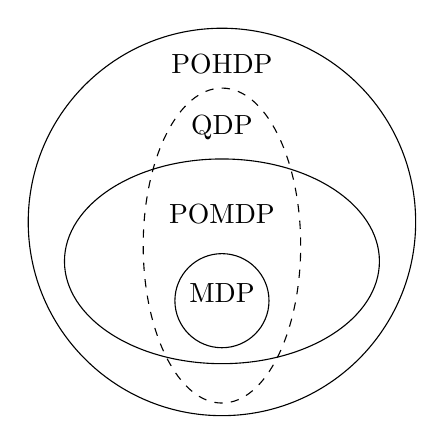
\begin{tikzpicture}
    \draw (0,0) circle (70pt) ;
    \node at (0,2) { POHDP };
    \draw (0,-0.5) circle [x radius = 2cm, y radius = 1.3cm]; % (40pt) ;
    \node at (0,0.1) { POMDP };
    \draw (0,-1) circle (17pt) ;
    \node at (0,-0.9) { MDP };
    \draw[dashed] (0, -0.3) circle [x radius=1cm, y radius=2cm];
    \node at (0,1.2) { QDP };
  \end{tikzpicture}
  \caption{Classes of finite decision processes considered in \ncite{MH18},
    under \cref{sett:HDP_MH}
    (recall that QDP is a partially observable HDP under state-uniformity
    \cref{asm:stateUniformity}).
  }
  \label{fig:DPMH}
\end{figure}

\begin{rem}
 It remains unclear after reading \ncite{MH18}
why $q^*$ and $Q^*$ are well defined as the solution to their
functional equations (\cref{eq:MH_Q_def} and \cref{eq:MH_q_def})
and how are they related to the optimal value function
$V^*(s) = \sup_{\pi \in R\Pi} \E_s^\pi
\sum_{i=1}^\infty \gamma^{i-1} r_i $
(see \cref{defn:optimalValue})
of a general HDP?
A sensible thing to ask would be that
$Q^*(h, a) = r(h, a) + \gamma \E_{P(\cdot \mid h a)} V^*$.
An analysis of this could have been made by generalizing the results
on Q-functions of section 2.
The main discussion of Q-functions in this thesis have been aimed at
MDPs since most results are in this setting,
and we will not go further into these details.
Alternatively a further study into the articles of Hutter
(and associated authors) might also gives such insights. 
\end{rem}

With this we conclude our section on finite decision processes and turn
to processes with continuous state spaces.

\section{Linear function approximation} \label{sec:linearFunctionApprox}

In this section we will look at a general method of approximation of
Q-functions,
namely approximation by a linear span from a set of basis functions.
This was investigated by \mcite{MR07} on which is section is based.

\begin{sett}[Continuous state, finite action, discounted MDP]
  \leavevmode
  \begin{enumerate}
    \item An MDP $(\cl{S}, \cl{A}, P, R, \gamma)$ (see \cref{sett:MDP}).
    \item $\cl{S} \subseteq \R^w$ is a compact subset of a euclidean space.
    \item $\cl{A}$ is finite and unrestricted, that
      is $\frak{A}(s) = \cl{A}$ for all 
      $s \in \cl{S}$.
    \item $r_i$ is upper semicontinuous \label{item:MRlast}.
  \end{enumerate}
  \label{sett:MR}
\end{sett}

\begin{rem}
  \Cref{item:MRlast} was actually not part of the assumptions in
  \ncite{MR07}.
  We include it here in order to ensure the existence of an
  optimal policy and thus measurability of $V^*$.
\end{rem}

Let $\left\{ \xi_1, \dots, \xi_M \right\}$ be a finite set of linearly
independent, measurable and bounded Q-functions,
$\xi_i : \cl{S} \times \cl{A} \to \R,\; \forall i \in [M]$.
Denote $\cl{F} \defeq \Span\left\{ \xi_i \mid i \in [M] \right\}$
and for $\theta \in \R^M$
\begin{equation}
  Q_\theta(s, a) = \sum_{i=1}^M \theta_i \xi_i(s, a) = \xi^T \theta
  \label{eq:QthetaLinApprox}
\end{equation}
where we view $\xi = (\xi_1, \dots, x_M) : \cl{S} \times \cl{A} \to \R^M$
as the combined \emph{vector} function, and $\xi^T$ is transposition
so that $\xi^T \theta$ is another way of writing the standard inner (dot)
product.

Note that $\cl{F} \subseteq \cl{L}_2(\cl{S}\times\cl{A})$ since any
$Q_\theta$ is bounded and $\cl{S}$ is compact (so closed and bounded).
We would now like to find the best approximation
$q^* \in \cl{F}$ to $Q^*$ within the span.
If we measure distance by the $\cl{L}_2$-norm this is
simply $q^* = \rho_\cl{F} Q^*$ where $\rho_\cl{F}$ is the orthogonal projection on
$\cl{F}$. Denote by $\theta^*$ the coordinates of this projection, i.e.
$q^* = Q_{\theta^*} = \rho_\cl{F} Q^*$.

It is easily seen that the gradient of $Q_\theta$ over $\theta$ is
$\nabla_\theta Q_\theta = \xi$.
This gives the idea for a temporal difference term with approximation from
$\cl{F}$ using the update step.
Let $(s_1, a_1, s_2, a_2, \dots) \in \cl{S} \times \cl{A} \times \cl{S} \times
\dots$ be states and actions sampled from
an decision process when we could use the following update on our
parameters:
\begin{equation}
  \theta_{k+1} = \theta_k + \alpha_k \xi(s_k, a_k)
  \left( r_k + \gamma \max_{b \in \cl{A}} Q_{\theta_k}(s_{k+1}, b)
- Q_{\theta_k}(s_k, a_k) \right)
\label{eq:linApproxUpdateStep}
\end{equation}

\begin{figure}[H]
\begin{algorithm}[H] %\label{algocf:fq} % this labels line, could not fix
  \caption{Q-learning with linear approximation}
  \KwIn{MDP $(\cl{S}, \cl{A}, P, R, \gamma)$,
    policy $\pi \in R\Pi$,
    number of iterations $K$,
    learning rates $(\alpha_1, \dots, \alpha_K)$,
    initial $\theta_1 \in \R^M$
  }

  \For{$k = 1,2,\dots,K$}{
    Sample $a_k \sim \pi(\cdot \mid s_k)$,
    $s_{k+1} \sim P(\cdot \mid s_k, a_k)$,
    $r_k \sim R(\cdot \mid s_k, a_k)$.

    Update action-value parameter:
    \[ \theta_{k+1} = \theta_k + \alpha_k \xi(s_k, a_k)
      \left( r_k + \gamma \max_{b \in \cl{A}} Q_{\theta_k}(s_{k+1}, b)
    - Q_{\theta_k}(s_k, a_k) \right) \]
  }
  Define $\wt{\pi}_K$ as the greedy policy w.r.t.
  $\wt{Q}_K \defeq Q_{\theta_{K+1}}$.

  \KwOut{An estimator $\wt{Q}_K$ of $Q^*$ and policy $\wt{\pi}_K$}
  \label{alg:QLlinear}
\end{algorithm}
\end{figure}
The policy given as input to this algorithm, may depend on the history
and should be seen as a way of sampling from $\cl{A}$, rather than
a effective strategy. The main point in this section is to show convergence,
so we are 
interested in a policy providing sufficient support of the distributions
of the samples $(s_i, a_i)$ across $\cl{S} \times \cl{A}$.
This is made precise by the assumptions of \emph{ergodicity} on the process.

We can view an MDP as a stationary process $\fk{P}$ on $\cl{S}$
generated by kernel $P\pi$ for a policy $\pi \in S\Pi$.
This makes sense to the property of ergodicity for the process
which can be viewed as the continuous state-space equivalent of
the requirement that every state and action is visited infinitely often
in the finite MDPs.
For a full definition of \emph{geometric ergodicity}, which we will need
in the following main result from \ncite{MR07}, see \cref{sec:geometricErgo}.

\begin{thm}[Melo, Ribeiro]
  Let $(\cl{S}, \cl{A}, P, R, \gamma)$ be an MDP as of \cref{sett:MR}.
  Let $\pi \in S\Pi$ be a stationary process
  and $\fk{P}$ the process kernel derived by $P\pi$.
  Assume that $\fk{P}$ is geometrically
  ergodic\footnote{See \cref{sec:geometricErgo}.} with invariant
  measure $\mu$ and that
  $\pi(a \mid s) > 0$ for all $a \in \cl{A}$ and $\mu$-almost all
  $s \in \cl{S}$.
  Assume that $\sum_{i=1}^M \abs{\xi_i} \leq 1$.
  Then if \cref{alg:QLlinear} is run with learning rates from a sequence
  $\{ \alpha_k \}_{k \in \N}$ satisfying $\alpha_k \in [0,1]$ and
  \[ \sum_{k = 1}^\infty \alpha_k = \infty, \qquad
  \sum_{k = 1}^\infty \alpha_k^2 < \infty \]
  we have that
  \[ \theta_k \to \theta^* \]
  with probability 1, and $Q_{\theta^*}$ satisfies
  \[ Q_{\theta^*} = \rho_\cl{F} T Q_{\theta^*} \]
  Furthermore the orthogonal projection is expressible as
  \[ \rho_\cl{F} Q = \xi^T
    \frac{\E_{\pi\mu}\left( \xi Q \right)}{\E_{\pi\mu} (\xi \xi^T)}
  \]
  \label{thm:MeloRibeiro}
\end{thm}
\begin{rem}
  Recall the definition of the kernel-derived measure $\pi \mu(S \times A)
  = \int_S \pi(A \mid s) \difd \mu(s)$ (see \cref{thm:intKer}).
\end{rem}

The theorem \ref{thm:MeloRibeiro} by Melo and Ribeiro
shows that Q-learning still works when using a gradient step
version of the temporal difference update in a continuous state space setting,
and it guarantees convergence to optimality within the approximating function
class.
However there is still room for improvement since \cref{thm:MeloRibeiro}
does not tell us:
\begin{center}
\begin{enumerate*}[itemjoin=\hspace{0.3in}]
  \item How fast is the convergence?
  \item How far is $Q_{\theta^*}$ from $Q^*$?
    \label{item:linApprox1}
  \item How far is $Q_{\wt{\pi}_K}$ from $Q^*$?
\end{enumerate*}
\end{center}
\begin{rem}
  Question 2. is probably best handled seperately for each
    function class $\cl{F}$.
\end{rem}
In a quite similar setting these questions are answered for the
fitted Q-iteration algorithm in the next section (\cref{thm:main}).

